\documentclass[manuscript]{acmart}

\setcopyright{none}
\acmJournal{TOMS}
\acmYear{2026}
\citestyle{acmauthoryear}

\usepackage{amsfonts}
\usepackage{amsthm}
\usepackage{mathtools}
\usepackage{tabularx,array,longtable}
\usepackage[ruled,vlined,linesnumbered]{algorithm2e}
\usepackage[shortlabels]{enumitem}

\theoremstyle{plain}
\newtheorem{theorem}{Theorem}[section]
\newtheorem{lemma}[theorem]{Lemma}
\newtheorem{proposition}[theorem]{Proposition}
\newtheorem{corollary}[theorem]{Corollary}
\theoremstyle{definition}
\newtheorem{definition}[theorem]{Definition}
\newtheorem{example}[theorem]{Example}
\newtheoremstyle{nonitalicremark}
  {6pt}{6pt}% Space above/below
  {\normalfont}% Body font
  {}% Indent amount
  {\bfseries}% Head font
  {.}% Punctuation after head
  {.5em}% Space after head
  {}% Head spec
\theoremstyle{nonitalicremark}
\newtheorem{remark}[theorem]{Remark}

\newcommand{\Q}{\mathbb{Q}}
\newcommand{\R}{\mathbb{R}}
\newcommand{\Z}{\mathbb{Z}}
\newcommand{\OO}{\mathcal{O}}
\newcommand{\OD}{\OO_D}
\newcommand{\Tr}{\operatorname{Tr}}
\newcommand{\N}{\operatorname{N}}
\newcommand{\Disc}{\operatorname{Disc}}
\newcommand{\covol}{\operatorname{covol}}
\newcommand{\eps}{\varepsilon}
\newcommand{\into}{\hookrightarrow}
\newcommand{\cP}{\mathcal{P}}
\newcommand{\cE}{\mathcal{E}}
\newcommand{\cB}{\mathcal{B}}
\newcommand{\cQ}{\mathcal{Q}}
\newcommand{\cR}{\mathcal{R}}
\newcommand{\cS}{\mathcal{S}}
\newcommand{\cW}{\mathcal{W}}
\newcommand{\cT}{\mathcal{T}}
\graphicspath{{figures/}}

\title[Exact diagonal representability over real quadratic orders]{Exact diagonal representability over real quadratic orders via weighted trace-form enumeration}

\author{Tomasz Kania}
\authornote{IM CAS (RVO 67985840).}
\affiliation{%
  \institution{Institute of Mathematics, Czech Academy of Sciences}
  \city{Prague}
  \country{Czech Republic}}
\affiliation{%
  \institution{Institute of Mathematics, Jagiellonian University}
  \city{Krak\'ow}
  \country{Poland}}
\email{tomasz.marcin.kania@gmail.com}

\begin{document}

\begin{abstract}
\texttt{quadratic\_diagonal} is a self-contained pure-Python reference package for exact
constructive representability by diagonal quadratic lattices over maximal real quadratic orders.
Given a squarefree radicand, totally positive diagonal coefficients, and a totally positive target,
the software decides representability and returns an integral witness when one exists. The package
implements weighted trace-form enumeration, dynamic-programming and meet-in-the-middle solvers,
and batched bounded search for representable targets and bounded truants. The accompanying article
proves the weighted discriminant identity, the distinct-value asymptotic, exact row-interval
correctness, and pseudo-polynomial arithmetic-step bounds for fixed fields and fixed lattices. All
comparisons in the core routines use integer trace and norm arithmetic; no floating-point boundary
or ordering tests are used. The repository contains the installable package, non-interactive drivers,
regression tests, validation sweeps, benchmark scripts, generated tables, performance plots, and an
executed notebook. The implementation is intended both as a reusable research tool and as an
executable specification that can be translated into compiled code or integrated into SageMath-style
Python workflows.
\end{abstract}


\ccsdesc[500]{Mathematics of computing~Mathematical software}
\ccsdesc[300]{Mathematics of computing~Number theory}
\ccsdesc[300]{Mathematics of computing~Algebraic algorithms}
\ccsdesc[300]{Software and its engineering~Software libraries and repositories}

\keywords{algorithms, quadratic forms, real quadratic fields, rings of integers, diagonal representability, dynamic programming, mathematical software}

\maketitle

\section{Introduction}

This paper presents a self-contained software package and accompanying exact algorithms for
constructive representability by diagonal quadratic lattices over maximal real quadratic orders. The
package, \texttt{quadratic\_diagonal}, is intended as a transparent reference implementation: it
exposes a small exact API, ships with regression tests, benchmark scripts, performance plots, and an
executed notebook, and reproduces the tables and figures in Section~\ref{sec:impl} from the public
repository source tree. Python is used deliberately as an executable specification language: the
resulting code is easy to inspect, test, and translate, and it can be integrated directly into
SageMath-style Python workflows even when higher-performance compiled backends are ultimately
preferred.

The underlying mathematical problem is the following. Let
\[
L=\langle a_1,\dots,a_r\rangle,
\qquad a_i\in\OD^+,
\qquad \alpha\in\OD^+.
\]
We want to decide whether
\[
\alpha = a_1x_1^2+\cdots+a_rx_r^2
\qquad (x_1,\dots,x_r\in\OD),
\]
and, if so, to construct such a representation. The package API exposes an exact order
model and routines for weighted enumeration, constructive dynamic programming,
meet-in-the-middle search, and bounded-target batching; the README documents the
precise entry-point names and command-line reproduction scripts.

From the literature viewpoint, this work sits between algorithmic quadratic-form computation over
fields and arithmetic investigations over rings of integers. Koprowski and Czoga{\l}a developed
fundamental algorithms for quadratic forms over number fields, including isotropy, hyperbolicity,
level, Pythagoras number, Witt equivalence, and related tasks \cite{KopCz}. Koprowski and
Rothkegel later gave an algorithm for constructing anisotropic parts over number fields
\cite{KopRoth}, while Koprowski subsequently provided explicit algorithms for sums of squares and
for isotropic vectors over arbitrary global fields \cite{KopSq,KopIso}. In the real-quadratic
integral setting, Ra\v ska studied when all elements of $m\OD^+$ are sums of squares and gave an
efficient algorithm for that family-wise question \cite{Raska}. The present repository is organised
in the same spirit as the author's companion public repository \texttt{quadratic\_sos} \cite{KaniaQSOS},
which treats the unweighted $\langle 1,\dots,1\rangle$ case. For broader arithmetic background on universal forms and
indecomposables over totally real fields we refer to Kala's survey \cite{KalaSurvey}; recent work
of Kala, Kr\'asensk\'y, and Romeo places criterion sets and diagonal universality in a general
framework \cite{KKR}, and their interaction with sums of squares has become more explicit in work
such as \cite{KKK}.

The novelty claim is deliberately narrow. We do \emph{not} claim a new lattice-enumeration method
in general. Rather, we specialise classical exact lattice enumeration to the weighted trace form
over maximal real quadratic orders, make the resulting implementation fully exact and self-contained,
integrate it with constructive diagonal representability, and strengthen the bounded-target layer by
a batched dynamic program. The software contribution is as important here as the theorem statements:
the package is installable, the public API mirrors the mathematical objects proved in the paper, the
computational section is regenerated from scripts and notebook cells shipped in the repository, and
we include a reproducible generic exact baseline in order to evaluate the specialised solvers against
a direct value-product search.

The first main point is that the weighted trace form carries more structure than a generic box bound
reveals. If
\[
q_a(m+n\omega_D)=A_am^2+B_amn+C_an^2,
\]
then its discriminant parameter is not merely positive; it is exactly
\[
4A_aC_a-B_a^2 = 4\Disc(K_D)\N(a).
\]
This identity gives the exact area of the trace ellipse and, after quotienting by the sign symmetry
$x\sim -x$, the correct leading constant for the number of \emph{distinct weighted values}. The
second main point is algorithmic: the exact search can be organised over a canonical half-ellipse,
so that the implementation visits exactly one representative from each non-zero $\pm$-pair of roots
and stores only one witness root per distinct value. The third main point is bounded search: for a
trace bound $B$, all representable targets of trace at most $B$ can be computed in one batched
pass, rather than by rerunning the representability solver for each target separately.

Our main contributions are these.
\begin{enumerate}[label=\textup{(N\arabic*)},itemsep=0.25em]
\item We prove the discriminant identity for the weighted trace form, the resulting area formula for
the trace ellipse, and the corresponding asymptotic for distinct weighted values of bounded trace.
\item We give an exact ellipse-sensitive weighted search which enumerates $\cS_a(\alpha)$ by row
intervals of the trace ellipse, scans only a canonical half-ellipse, and uses only integer arithmetic
and exact comparisons in $\OD$.
\item We give exact constructive dynamic-programming and meet-in-the-middle algorithms for diagonal
representability by $\langle a_1,\dots,a_r\rangle$, record permutation invariance, exploit internal
coefficient reordering and repeated-coefficient caching in the implementation, and deduce a
pseudo-polynomial bound for single targets via the dynamic-programming method.
\item We give an exact batched bounded representability algorithm and deduce a pseudo-polynomial
$O(B^3)$ bound for bounded truants over a fixed field and a fixed diagonal lattice.
\item We provide a self-contained Python package, regression tests, benchmark tables, performance
plots, and an executed notebook reporting meaningful structural quantities: distinct weighted values,
canonical candidate counts, DP state sizes, half-sum sizes, coefficient-order effects,
repeated-coefficient caching gains, and split preprocessing, combination, and end-to-end timings.
\end{enumerate}

\subsection*{Software availability and reproducibility}

The public repository associated with this paper will be maintained at
\url{https://github.com/tomaszkania/quadratic_diagonal}; the submission bundle contains the same
source tree. The top-level package \texttt{quadratic\_diagonal} is installable with
\texttt{pip install -e .} and exposes the exact API used throughout the paper. The repository also
contains regression tests, a validation sweep, the script \path{scripts/reproduce_tables.py},
which regenerates all TSV tables in \path{data/} together with the performance plots in
\path{paper/figures/}, and the executed notebook \path{notebooks/paper_illustrations.ipynb}.
The structural columns in the computational section are deterministic; only the timing columns are
machine-dependent.

For a TOMS Algorithm-paper submission the software component is supplied as a separate archive in
the repository's \path{submission/} directory. That archive contains the installable source package,
non-interactive driver programs, regression and validation tests, expected-output summaries, table
and figure reproduction scripts, a manifest, and portability notes. The smoke-test driver
\path{scripts/run_all_checks.py} requires no interactive input and is intended as the first command
for referees; it exercises the public API, checks the regression suite, regenerates deterministic
structural data, and records timing-dependent quantities separately.

The organisation is as follows. Section~\ref{sec:prelim} recalls exact arithmetic in $\OD$ and the
trace-norm comparison lemma used in the implementation. Section~\ref{sec:weighted} studies the
weighted trace form, proves the discriminant identity, and derives the ellipse-area and lattice-point
asymptotic formulas. Section~\ref{sec:search} gives the exact weighted search on a canonical
half-ellipse and its ellipse-sensitive complexity. Section~\ref{sec:repr} develops the constructive
DP and meet-in-the-middle layers, records unit-square invariance, and proves the single-target
pseudo-polynomial bound. Section~\ref{sec:bounded} replaces per-target bounded search by a batched
dynamic program and proves the bounded pseudo-polynomial complexity bound. Section~\ref{sec:impl}
describes the software artefact, the reproducibility workflow, a generic exact baseline comparison,
the benchmark data, the performance plots, and a short arithmetic case study. The degree-$2$
restriction is essential to the present geometry: over a totally real field of degree $d$ the
weighted trace form becomes a positive-definite lattice problem in rank $d$, so for cubic fields the
search region is a genuine ellipsoid in $\R^3$ and the exact row-interval formulas used here no
longer collapse to one-dimensional arithmetic.

\section{Preliminaries}\label{sec:prelim}

Let $D\ge 2$ be squarefree and write
\[
K_D=\Q(\sqrt D),
\qquad
\OD=\OO_{K_D}.
\]
We fix the standard integral generator
\[
\omega_D=
\begin{cases}
\sqrt D, & D\equiv 2,3 \pmod 4,\\[0.3em]
\dfrac{1+\sqrt D}{2}, & D\equiv 1 \pmod 4,
\end{cases}
\]
so that $\OD=\Z[\omega_D]$. Every element of $\OD$ is written uniquely as $a+b\omega_D$ with
$a,b\in\Z$, and we identify it with the coefficient pair $(a,b)\in\Z^2$. We restrict throughout to
the maximal order because this keeps both the coordinate model and the trace--norm comparison
formulas uniform; extending the same exact algorithms to non-maximal orders would require additional
bookkeeping for the conductor and the resulting coordinate constraints.

The two real embeddings are denoted by
\[
\sigma_1,\sigma_2:K_D\into\R,
\qquad
\sigma_1(\sqrt D)=\sqrt D,
\qquad
\sigma_2(\sqrt D)=-\sqrt D.
\]
We write $x\preccurlyeq y$ if $\sigma_i(x)\le \sigma_i(y)$ for $i=1,2$, and $x\prec y$ if both
inequalities are strict. Throughout, undecorated symbols such as $\leq$ and $<$ refer to the usual
order on $\Z$ or $\R$.

\begin{lemma}\label{lem:trace-norm}
For every $z\in K_D$ one has:
\begin{enumerate}[label=\textup{(\roman*)}]
\item $z\succcurlyeq 0$ if and only if $\Tr(z)\ge 0$ and $\N(z)\ge 0$;
\item $z\succ 0$ if and only if $\Tr(z)>0$ and $\N(z)>0$.
\end{enumerate}
\end{lemma}

\begin{proof}
Write $z_i=\sigma_i(z)$. Then $\Tr(z)=z_1+z_2$ and $\N(z)=z_1z_2$. If $z_1,z_2\ge 0$, then both
quantities are non-negative. Conversely, $z_1$ and $z_2$ are the roots of
\[
t^2-\Tr(z)\,t+\N(z)=0.
\]
If $\Tr(z)\ge 0$ and $\N(z)\ge 0$, then the sum and product of the roots are both non-negative, so
the two roots are either both non-negative or both non-positive; the non-negative sum rules out the
second possibility. Hence $z_1,z_2\ge 0$. This proves \textup{(i)}. The proof of \textup{(ii)} is
identical, with strict inequalities.
\end{proof}

\begin{corollary}\label{cor:comparison}
For $x,y\in K_D$ one has
\[
x\preccurlyeq y
\iff
\Tr(y-x)\ge 0\text{ and }\N(y-x)\ge 0.
\]
Likewise,
\[
x\prec y
\iff
\Tr(y-x)>0\text{ and }\N(y-x)>0.
\]
\end{corollary}

\begin{proof}
Apply Lemma~\ref{lem:trace-norm} to $y-x$.
\end{proof}

\begin{definition}
For $x\in\OD$, write $x\in\OD^+$ if $x\succ 0$. A diagonal $\OD$-lattice is an expression
\[
L=\langle a_1,\dots,a_r\rangle,
\qquad a_i\in\OD^+.
\]
We say that $\alpha\in\OD^+$ is represented by $L$, and write $\alpha\to L$, if there exist
$x_1,\dots,x_r\in\OD$ such that
\[
\alpha=a_1x_1^2+\cdots+a_rx_r^2.
\]
\end{definition}

If $D\equiv 1\pmod 4$, then
\[
\omega_D^2=\omega_D+\frac{D-1}{4},
\]
while for $D\equiv 2,3\pmod 4$ one has $\omega_D^2=D$. The trace and norm of $a+b\omega_D$ are therefore
\[
\Tr(a+b\omega_D)=
\begin{cases}
2a+b, & D\equiv 1\pmod 4,\\
2a, & D\equiv 2,3\pmod 4,
\end{cases}
\]
and
\[
\N(a+b\omega_D)=
\begin{cases}
a^2+ab-\dfrac{D-1}{4}b^2, & D\equiv 1\pmod 4,\\
a^2-Db^2, & D\equiv 2,3\pmod 4.
\end{cases}
\]

\section{Weighted trace forms and their geometry}\label{sec:weighted}

Fix $a\in\OD^+$ and define the weighted trace form
\[
q_a(x)=\Tr(a x^2)
\qquad (x\in\OD).
\]
Writing $x=m+n\omega_D$ with $m,n\in\Z$ yields an integral binary quadratic form
\[
q_a(m+n\omega_D)=A_am^2+B_amn+C_an^2
\qquad (A_a,B_a,C_a\in\Z).
\]

\begin{proposition}\label{prop:positive-definite}
For every $a\in\OD^+$, the form $q_a$ is a positive definite integral binary quadratic form on the
lattice $\OD\cong\Z^2$.
\end{proposition}

\begin{proof}
For every $x\in\OD$ we have $a x^2\in\OD$, hence $q_a(x)=\Tr(a x^2)\in\Z$. If $x\ne 0$, then
\[
q_a(x)=\sigma_1(a)\sigma_1(x)^2+\sigma_2(a)\sigma_2(x)^2.
\]
Since $a\in\OD^+$, both coefficients are strictly positive, and the two squares are non-negative and
not both zero. Thus $q_a(x)>0$ for every non-zero $x$.
\end{proof}

\begin{definition}
Let
\[
\delta_a = 4A_aC_a-B_a^2.
\]
Since $q_a$ is positive definite, one has $A_a>0$, $C_a>0$, and $\delta_a>0$.
\end{definition}

\begin{theorem}[Discriminant identity]\label{thm:disc-id}
Let $\Disc(K_D)$ denote the field discriminant of $K_D$. Then
\[
\delta_a = 4\Disc(K_D)\N(a).
\]
\end{theorem}

\begin{proof}
Let $e_1=1$ and $e_2=\omega_D$, and consider the symmetric bilinear form
\[
T_a(x,y)=\Tr(a x y)
\qquad (x,y\in K_D).
\]
Its Gram matrix in the basis $(e_1,e_2)$ is
\[
G_a = \bigl(T_a(e_i,e_j)\bigr)_{i,j=1}^2.
\]
If
\[
E=\begin{pmatrix}
\sigma_1(e_1) & \sigma_1(e_2)\\
\sigma_2(e_1) & \sigma_2(e_2)
\end{pmatrix},
\]
then entrywise one has
\[
G_a = E^{\top}
\begin{pmatrix}
\sigma_1(a) & 0\\ 0 & \sigma_2(a)
\end{pmatrix}
E.
\]
Indeed,
\[
T_a(e_i,e_j)=\sigma_1(a)\sigma_1(e_i)\sigma_1(e_j)+\sigma_2(a)\sigma_2(e_i)\sigma_2(e_j).
\]
Therefore
\[
\det G_a = \sigma_1(a)\sigma_2(a)\, (\det E)^2 = \N(a)\,(\det E)^2.
\]
For $a=1$ this becomes the Gram matrix of the trace pairing on the integral basis $(1,\omega_D)$, so
\[
(\det E)^2 = \det G_1 = \Disc(K_D).
\]
Since $T_a(x,x)=\Tr(a x^2)=q_a(x)$, the diagonal entries of $G_a$ are $A_a$ and $C_a$, while the
off-diagonal entry is $B_a/2$. On the other hand,
\[
G_a = \begin{pmatrix}
A_a & B_a/2\\ B_a/2 & C_a
\end{pmatrix},
\]
whence
\[
\det G_a = A_aC_a-\frac{B_a^2}{4}=\frac{\delta_a}{4}.
\]
Combining the two determinant formulas yields the claim.
\end{proof}

\begin{corollary}[Ellipse area]\label{cor:ellipse-area}
For $T>0$, let
\[
\cE_a(T)=\{(m,n)\in\R^2 : q_a(m+n\omega_D)\le T\}.
\]
Then
\[
\operatorname{area}(\cE_a(T)) = \frac{\pi T}{\sqrt{\Disc(K_D)\N(a)}} = \frac{2\pi T}{\sqrt{\delta_a}}.
\]
\end{corollary}

\begin{proof}
Let
\[
M_a=\begin{pmatrix}A_a & B_a/2\\ B_a/2 & C_a\end{pmatrix}.
\]
Then $q_a(m+n\omega_D)=(m,n)M_a(m,n)^{\top}$. Since $M_a$ is positive definite, the change of
variables $y=M_a^{1/2}x$ sends $\cE_a(T)$ to the Euclidean disk of radius $\sqrt T$. Thus
\[
\operatorname{area}(\cE_a(T)) = \frac{\pi T}{\sqrt{\det M_a}}.
\]
Now $\det M_a=\delta_a/4$ and Theorem~\ref{thm:disc-id} gives $\delta_a=4\Disc(K_D)\N(a)$.
\end{proof}

\begin{corollary}[Candidate asymptotic]\label{cor:candidate-asymptotic}
Let
\[
M_a(T)=\#\bigl(\cE_a(T)\cap\Z^2\bigr).
\]
Then
\[
M_a(T)=\frac{\pi T}{\sqrt{\Disc(K_D)\N(a)}} + O_a(\sqrt T).
\]
In particular, for fixed $a$ one has $M_a(T)=\Theta_a(T)$.
\end{corollary}

\begin{proof}
A standard lattice-point estimate for bounded convex planar regions with smooth boundary gives
\[
\#(\Lambda\cap C)=\frac{\operatorname{area}(C)}{\covol(\Lambda)}+O\bigl(\operatorname{perimeter}(C)+1\bigr)
\]
for each translate of a full-rank lattice $\Lambda\subseteq\R^2$; see, for instance,
\cite[Chapter~2]{GruberLekkerkerker}. Here $\Lambda=\Z^2$ has covolume $1$, and
$\cE_a(T)$ is an ellipse with perimeter $O_a(\sqrt T)$. The claim now follows from
Corollary~\ref{cor:ellipse-area}.
\end{proof}

\section{Exact weighted search}\label{sec:search}

Fix $a,\alpha\in\OD^+$ and set $T=\Tr(\alpha)$. Define the weighted root and value sets
\[
\cR_a(\alpha)=\{x\in\OD\setminus\{0\} : a x^2\preccurlyeq \alpha\},
\qquad
\cS_a(\alpha)=\{a x^2 : x\in\cR_a(\alpha)\}.
\]
Since $a\in\OD^+$, every non-zero value $a x^2$ is automatically totally positive. We also define
the canonical root set
\[
\cR_a^+(\alpha)=\{m+n\omega_D\in\cR_a(\alpha) : n>0\text{ or }(n=0,\ m>0)\}.
\]
Thus $\cR_a^+(\alpha)$ contains exactly one representative from each non-zero sign pair. We call the
elements of $\cR_a^+(\alpha)$ the \emph{canonical candidates} for the weighted search set.

\begin{lemma}\label{lem:two-to-one}
If $a\in\OD\setminus\{0\}$ and $x,y\in\OD\setminus\{0\}$ satisfy $a x^2=a y^2$, then $y=\pm x$.
Consequently, the map $x\mapsto a x^2$ is exactly two-to-one on non-zero roots, and its restriction
\[
\cR_a^+(\alpha)\to\cS_a(\alpha)
\]
is a bijection. In particular,
\[
\#\cR_a(\alpha)=2\#\cS_a(\alpha),
\qquad
\#\cR_a^+(\alpha)=\#\cS_a(\alpha).
\]
\end{lemma}

\begin{proof}
Since $\OD$ is an integral domain of characteristic $0$, the equality $a x^2=a y^2$ implies
$x^2=y^2$, hence $(x-y)(x+y)=0$. Thus $y=\pm x$. Conversely, $x$ and $-x$ clearly yield the same
weighted square.

It remains to show that every non-zero sign pair $\{x,-x\}$ contains exactly one element of the
canonical half. Write $x=m+n\omega_D$. If $n\neq 0$, then exactly one of $n$ and $-n$ is positive.
If $n=0$, then $m\neq 0$, so exactly one of $m$ and $-m$ is positive. Therefore $\{x,-x\}$ meets
$\cR_a^+(\alpha)$ in exactly one element. The bijectivity of the restricted map follows.
\end{proof}

\begin{corollary}[Distinct-value asymptotic]\label{cor:distinct-asymptotic}
For fixed $a\in\OD^+$ and $B>0$ one has
\[
\#\{a x^2\in\OD^+ : 0<\Tr(a x^2)\le B\}
=
\frac{\pi B}{2\sqrt{\Disc(K_D)\N(a)}} + O_a(\sqrt B).
\]
\end{corollary}

\begin{proof}
Let $M_a(B)=\#(\cE_a(B)\cap\Z^2)$ as in Corollary~\ref{cor:candidate-asymptotic}. The lattice point
$(0,0)$ belongs to $\cE_a(B)$, so $M_a(B)-1$ is the number of non-zero roots satisfying
$\Tr(a x^2)\le B$. By Lemma~\ref{lem:two-to-one}, the number of distinct weighted values is exactly
$(M_a(B)-1)/2$. The result follows from Corollary~\ref{cor:candidate-asymptotic}.
\end{proof}

\begin{lemma}\label{lem:trace-necessary}
If $x\in\cR_a(\alpha)$, then $q_a(x)\le T$.
\end{lemma}

\begin{proof}
If $x\in\cR_a(\alpha)$, then $a x^2\preccurlyeq \alpha$. Summing the two embedding inequalities gives
\[
\Tr(a x^2)\le \Tr(\alpha)=T.
\]
\end{proof}

\begin{proposition}[Exact row interval]\label{prop:row-interval}
Fix $n\in\Z$. Set
\[
\Delta_n = 4A_a T - \delta_a n^2,
\qquad
m_n^-(\alpha)=\left\lceil \frac{-B_a n - \lfloor\sqrt{\Delta_n}\rfloor}{2A_a} \right\rceil,
\qquad
m_n^+(\alpha)=\left\lfloor \frac{-B_a n + \lfloor\sqrt{\Delta_n}\rfloor}{2A_a} \right\rfloor,
\]
whenever $\Delta_n\ge 0$. If $\Delta_n<0$, then the row is empty. If $\Delta_n\ge 0$, then the integers
$m$ satisfying
\[
A_a m^2+B_a m n + C_a n^2 \le T
\]
form the integer interval
\[
I_n(\alpha)=\bigl[m_n^-(\alpha), m_n^+(\alpha)\bigr]\cap\Z,
\]
which may still be empty. In the case $\Delta_n\ge 0$, the row is non-empty if and only if
$m_n^-(\alpha)\le m_n^+(\alpha)$.
\end{proposition}

\begin{proof}
A direct calculation gives
\[
4A_a\bigl(A_a m^2+B_a m n + C_a n^2\bigr) = (2A_a m + B_a n)^2 + \delta_a n^2.
\]
Hence the inequality is equivalent to
\[
(2A_a m + B_a n)^2 \le 4A_a T - \delta_a n^2 = \Delta_n.
\]
If $\Delta_n<0$, there is no solution. Otherwise set $s_n=\lfloor\sqrt{\Delta_n}\rfloor$. Since
$2A_a m + B_a n$ is an integer, the inequality above is equivalent to
\[
-s_n \le 2A_a m + B_a n \le s_n,
\]
which yields the stated interval after division by $2A_a>0$. The interval may still be empty if the
ceiling endpoint exceeds the floor endpoint, and this is exactly the criterion
$m_n^-(\alpha)\le m_n^+(\alpha)$ for row non-emptiness when $\Delta_n\ge 0$.
\end{proof}

\begin{remark}\label{rem:row-congruence}
The condition $\Delta_n\ge 0$ is only a necessary discriminant condition for row non-emptiness. Even
when $\Delta_n>0$, the congruence class of $B_a n$ modulo $2A_a$ can prevent the admissible interval
from containing an integer if the interval is too short.
\end{remark}

\begin{corollary}\label{cor:row-bound}
If $I_n(\alpha)\neq\varnothing$, then
\[
|n|\le \left\lfloor \sqrt{\frac{4A_a T}{\delta_a}}\right\rfloor.
\]
\end{corollary}

\begin{proof}
If $I_n(\alpha)$ is non-empty, then $\Delta_n\ge 0$. Hence $\delta_a n^2\le 4A_a T$.
\end{proof}

\begin{algorithm}[H]
\caption{ExactWeightedSearch$(a,\alpha)$}
\KwIn{A totally positive coefficient $a\in\OD^+$ and target $\alpha\in\OD^+$.}
\KwOut{The distinct values $\cS_a(\alpha)$ and one witness root for each value.}
Compute the weighted trace form $q_a(m+n\omega_D)=A_am^2+B_amn+C_an^2$\;
Set $T\leftarrow \Tr(\alpha)$ and $N\leftarrow \left\lfloor\sqrt{4A_aT/\delta_a}\right\rfloor$\;
Initialise an empty dictionary $\mathcal{V}$ from weighted values to roots\;
\For{$n=0$ \KwTo $N$}{
  Compute the exact row interval $I_n(\alpha)$ from Proposition~\ref{prop:row-interval}\;
  \If{$I_n(\alpha)$ is empty}{continue\;}
  Set $J_n\leftarrow I_n(\alpha)$\;
  \If{$n=0$}{replace $J_n$ by $J_n\cap\{1,2,3,\dots\}$\;}
  \For{$m\in J_n$}{
    Set $x\leftarrow m+n\omega_D$ and $s\leftarrow a x^2$\;
    \If{$s\preccurlyeq \alpha$}{store the pair $(s,x)$ in $\mathcal{V}$ if $s$ is not present\;}
  }
}
Return $\mathcal{V}$\;
\end{algorithm}

\begin{theorem}[Exact weighted search]\label{thm:weighted-search}
Algorithm~1 returns exactly the weighted value set $\cS_a(\alpha)$ together with one witness root for
each value.
\end{theorem}

\begin{proof}
Suppose the algorithm stores a value $s=a x^2$. Since $x\ne 0$ and $a\in\OD^+$, one has $s\succ 0$.
The acceptance test is $s\preccurlyeq \alpha$, so $x\in\cR_a(\alpha)$ and $s\in\cS_a(\alpha)$.

Conversely, let $s\in\cS_a(\alpha)$. Choose $x\in\cR_a(\alpha)$ with $s=a x^2$, and let $x^+$ be
the unique element of $\{x,-x\}\cap\cR_a^+(\alpha)$ given by Lemma~\ref{lem:two-to-one}. Then
$q_a(x^+)=q_a(x)\le T$ by Lemma~\ref{lem:trace-necessary}. Write $x^+=m+n\omega_D$. Since $x^+$ is
canonical, one has either $n>0$ or $n=0$ and $m>0$. Corollary~\ref{cor:row-bound} shows that the
algorithm reaches the row $n$, and Proposition~\ref{prop:row-interval} places $m$ inside the exact
row interval on that row. Thus the algorithm reaches $x^+$ and computes the same weighted value
$s=a(x^+)^2=a x^2$. Since $x^+\in\cR_a(\alpha)$, the acceptance test succeeds, so $s$ is stored.
\end{proof}

\begin{theorem}[Ellipse-sensitive complexity]\label{thm:candidate-sensitive}
Let
\[
M_a(\alpha)=\#\bigl(\cE_a(\Tr(\alpha))\cap\Z^2\bigr).
\]
Then Algorithm~1 scans exactly
\[
\frac{M_a(\alpha)-1}{2}
\]
canonical non-zero lattice points and performs
\[
O\bigl(M_a(\alpha)+\sqrt{\Tr(\alpha)}+1\bigr)
\]
exact arithmetic steps, up to the cost of hash-table operations. It stores exactly $\#\cS_a(\alpha)$
distinct weighted values and one witness root for each value. In particular, for fixed $a$ the
running time is $\Theta_a(\Tr(\alpha))$.
\end{theorem}

\begin{proof}
The algorithm scans precisely the rows with
\[
0\le n\le \left\lfloor \sqrt{\frac{4A_a\Tr(\alpha)}{\delta_a}}\right\rfloor,
\]
so the number of row computations is $O(\sqrt{\Tr(\alpha)}+1)$. On each scanned row,
Proposition~\ref{prop:row-interval} computes the exact interval in constant-time arithmetic. The
inner loop visits exactly the canonical non-zero lattice points in the trace ellipse
$\cE_a(\Tr(\alpha))$: for rows $n>0$ it scans the full integer interval, while on the central row it
keeps only positive abscissae. Every non-zero lattice point in the trace ellipse belongs to a unique
$\pm$-pair, and every such pair has exactly one canonical representative. Since $(0,0)$ is the only
fixed point of the sign involution, the number of scanned candidates is $(M_a(\alpha)-1)/2$.
Since the weighted values are stored as integer coefficient pairs whose coordinates are bounded by
$O(\Tr(\alpha))$, the hash-table insertions and lookups run in expected amortised constant time per
operation. The final statement follows from Corollary~\ref{cor:candidate-asymptotic}.
\end{proof}

\begin{remark}
All complexity statements in the paper are arithmetic-step bounds for exact integer operations. In a bit-complexity model one must additionally account for the growth of the integer coordinates and of the trace and norm computations, which are polynomial in the input size for fixed field and fixed lattice.
\end{remark}

\begin{remark}
Algorithm~1 is closely related to the Fincke--Pohst enumeration \cite{FinckePohst} specialised to a
rank-$2$ positive definite lattice. The additional features here are the canonical half-ellipse scan
of Lemma~\ref{lem:two-to-one}, which halves the non-zero candidate count, and the exact order
comparison in $\OD$, which keeps the implementation free of floating-point boundary tests.
\end{remark}

\begin{remark}\label{rem:trace-bounded-variant}
The same canonical row scan, with the final order-comparison filter removed, enumerates the trace-
bounded value set
\[
\{a x^2\in\OD^+ : 0<\Tr(a x^2)\le B\}
\]
in $O(B)$ time for fixed $a$.
\end{remark}

\section{Constructive diagonal representability}\label{sec:repr}

Fix a diagonal lattice
\[
L=\langle a_1,\dots,a_r\rangle,
\qquad a_i\in\OD^+,
\]
and a target $\alpha\in\OD^+$. For each $i$ set
\[
V_i(\alpha)=\{0\}\cup\cS_{a_i}(\alpha).
\]
The implementation stores one witness root for each non-zero value in $\cS_{a_i}(\alpha)$.

\begin{proposition}[Additive reduction]\label{prop:additive-reduction}
One has
\[
\alpha\to L
\iff
\alpha\in V_1(\alpha)+\cdots+V_r(\alpha).
\]
\end{proposition}

\begin{proof}
If
\[
\alpha=a_1x_1^2+\cdots+a_rx_r^2,
\]
then each summand is either $0$ or belongs to $\cS_{a_i}(\alpha)$, because every non-zero summand is
totally positive and bounded above by $\alpha$. Hence $\alpha$ lies in the displayed sumset.
Conversely, if
\[
\alpha=s_1+\cdots+s_r,
\qquad s_i\in V_i(\alpha),
\]
then for each non-zero $s_i$ choose the stored witness root $x_i$ with $s_i=a_i x_i^2$, and set
$x_i=0$ when $s_i=0$. Summing the resulting identities gives
\[
\alpha=a_1x_1^2+\cdots+a_rx_r^2,
\]
so $\alpha\to L$.
\end{proof}

\begin{proposition}[Permutation invariance]\label{prop:perm}
Let $\pi$ be a permutation of $\{1,\dots,r\}$. Then
\[
\alpha\to \langle a_1,\dots,a_r\rangle
\iff
\alpha\to \langle a_{\pi(1)},\dots,a_{\pi(r)}\rangle.
\]
\end{proposition}

\begin{proof}
The displayed equality
\[
\alpha=a_1x_1^2+\cdots+a_rx_r^2
\]
holds if and only if the same summands are written in the permuted order
\[
\alpha=a_{\pi(1)}x_{\pi(1)}^2+\cdots+a_{\pi(r)}x_{\pi(r)}^2.
\]
\end{proof}

\begin{remark}\label{rem:ordering}
Proposition~\ref{prop:perm} justifies reordering the coefficients internally. In the implementation
we sort the single-target value sets by non-decreasing $|\cS_{a_i}(\alpha)|$ and the bounded value
sets by non-decreasing $|\cW_i(B)|$ before the combination phase. We also cache repeated coefficients
so that each distinct weighted-value set is preprocessed only once.
\end{remark}

\begin{proposition}[Ordering upper bound]\label{prop:ordering-upper}
Let $s_i=\#\cS_{a_i}(\alpha)$ and, for a permutation $\pi$ of $\{1,\dots,r\}$, define
\[
U(\pi)=\sum_{j=1}^r \prod_{k=1}^j \bigl(s_{\pi(k)}+1\bigr).
\]
Then $U(\pi)$ is minimised when the sequence $s_{\pi(1)},\dots,s_{\pi(r)}$ is ordered
non-decreasingly.
\end{proposition}

\begin{proof}
It suffices to show that every adjacent inversion can be removed without increasing $U(\pi)$. Suppose
that for some $j$ one has
\[
s_{\pi(j)} > s_{\pi(j+1)}.
\]
Let $\pi'$ be obtained from $\pi$ by transposing $\pi(j)$ and $\pi(j+1)$. Then every prefix product
of length $<j$ is unchanged. The prefix product of length $j$ is multiplied by
\[
\frac{s_{\pi(j+1)}+1}{s_{\pi(j)}+1}<1,
\]
so it strictly decreases. Every later prefix product contains both factors
$s_{\pi(j)}+1$ and $s_{\pi(j+1)}+1$, hence is unchanged by the transposition. Thus
$U(\pi')\le U(\pi)$, with strict inequality unless the two adjacent factors are equal. Iterating
adjacent transpositions yields the non-decreasing ordering, which therefore minimises $U(\pi)$.
\end{proof}

\begin{proposition}[Repeated-coefficient caching]\label{prop:caching}
Suppose that the coefficient list $a_1,\dots,a_r$ assumes only $u$ distinct values.
With repeated-coefficient caching, the preprocessing stage for a single target $\alpha$ computes
exactly $u$ weighted search sets $\cS_a(\alpha)$, and the preprocessing stage for bounded search up
to trace bound $B$ computes exactly $u$ bounded weighted-value sets $\cW_a(B)$.
Consequently, for fixed field and fixed lattice, the preprocessing cost is
\[
O\bigl(u\,\Tr(\alpha)\bigr)
\]
for single targets and
\[
O(uB)
\]
for bounded batched search.
\end{proposition}

\begin{proof}
Caching identifies equal coefficients and stores one exact weighted enumeration for each distinct
coefficient value. Thus only $u$ weighted enumerations are performed. By
Theorem~\ref{thm:candidate-sensitive}, each single-target weighted search costs
$O(\Tr(\alpha))$ for fixed coefficient, and by Remark~\ref{rem:trace-bounded-variant} each bounded
weighted search costs $O(B)$ for fixed coefficient. Multiplying by the number $u$ of distinct
coefficients yields the stated bounds.
\end{proof}

\begin{definition}
Set $P_0(\alpha)=\{0\}$ and define recursively
\[
P_j(\alpha)=\{y+s : y\in P_{j-1}(\alpha),\ s\in V_j(\alpha),\ y+s\preccurlyeq \alpha\}
\qquad (1\le j\le r).
\]
\end{definition}

\begin{theorem}[Dynamic programming]\label{thm:dp}
For every $j$, the set $P_j(\alpha)$ is exactly the set of partial sums
\[
s_1+\cdots+s_j,
\qquad s_i\in V_i(\alpha),
\qquad s_1+\cdots+s_j\preccurlyeq \alpha.
\]
Consequently,
\[
\alpha\to L \iff \alpha\in P_r(\alpha).
\]
Moreover, if one stores one predecessor pair $(y,s)$ for each new element of $P_j(\alpha)$, then one
can reconstruct a representation whenever $\alpha\in P_r(\alpha)$.
\end{theorem}

\begin{proof}
The statement for $j=0$ is immediate. Assume it is true for $j-1$. By definition,
$P_j(\alpha)$ consists precisely of the sums of an element of $P_{j-1}(\alpha)$ and an element of
$V_j(\alpha)$ whose total remains bounded by $\alpha$. This is exactly the stated set of partial
sums. The equivalence with representability now follows from Proposition~\ref{prop:additive-reduction}.
The predecessor pointers record one such decomposition at every stage, so backtracking from
$\alpha\in P_r(\alpha)$ yields one tuple $(s_1,\dots,s_r)$ and hence one representing root tuple.
\end{proof}

\begin{corollary}[DP complexity and space]\label{cor:dp-complexity}
Let $s_j=\#\cS_{a_j}(\alpha)$. Then the dynamic-programming algorithm runs in
\[
O\!\left(\sum_{j=1}^r \#P_{j-1}(\alpha)\,(s_j+1)\right)
\]
exact arithmetic steps. The constructive implementation which stores predecessor maps for
backtracking uses
\[
O\!\left(\sum_{j=1}^r \#P_j(\alpha)\right)
\]
states, whereas a decision-only rolling-buffer variant uses
\[
O\!\left(\max_{0\le j\le r} \#P_j(\alpha)\right)
\]
states.
\end{corollary}

\begin{proof}
At layer $j$, every state in $P_{j-1}(\alpha)$ is combined with every candidate in $V_j(\alpha)$,
whose size is $s_j+1$. Each accepted sum is inserted into a hash table at most once, which yields
the time bound.

For the space bound, the constructive implementation stores one predecessor map for each layer
$j=1,\dots,r$, and the $j$th predecessor map has exactly $\#P_j(\alpha)$ entries. Thus the total
number of stored states is $\sum_{j=1}^r \#P_j(\alpha)$. If one only wants the decision problem, the
same recurrence can be run with two rolling buffers, storing only $P_{j-1}(\alpha)$ and $P_j(\alpha)$
at each step; this uses $O(\max_j \#P_j(\alpha))$ states.
\end{proof}

\begin{definition}
For $\alpha\in\OD^+$, let
\[
\cB(\alpha)=\{\beta\in\OD : 0\preccurlyeq \beta\preccurlyeq \alpha\}.
\]
\end{definition}

\begin{proposition}\label{prop:single-box-count}
Under the Minkowski embedding $\sigma:K_D\to\R^2$, the set $\cB(\alpha)$ corresponds to the lattice
$\sigma(\OD)$ intersected with the rectangle
\[
[0,\sigma_1(\alpha)]\times[0,\sigma_2(\alpha)].
\]
Consequently,
\[
\#\cB(\alpha)=\frac{\N(\alpha)}{\sqrt{\Disc(K_D)}} + O_D\bigl(\Tr(\alpha)\bigr).
\]
\end{proposition}

\begin{proof}
By definition, $0\preccurlyeq \beta\preccurlyeq \alpha$ if and only if both embedding coordinates of
$\sigma(\beta)$ lie in the stated rectangle. That rectangle has area
$\sigma_1(\alpha)\sigma_2(\alpha)=\N(\alpha)$ and perimeter
$2\sigma_1(\alpha)+2\sigma_2(\alpha)=2\Tr(\alpha)$. Since $\sigma(\OD)$ has covolume
$\sqrt{\Disc(K_D)}$, the standard planar lattice-point estimate used in
Corollary~\ref{cor:candidate-asymptotic} yields the formula.
\end{proof}

\begin{theorem}[Single-target pseudo-polynomial complexity]\label{thm:single-pseudopoly}
Fix the field $K_D$ and the diagonal lattice $L=\langle a_1,\dots,a_r\rangle$. Then the constructive
dynamic-programming algorithm decides whether $\alpha\to L$ and constructs a representation, when it
exists, in
\[
O\bigl((\N(\alpha)+\Tr(\alpha))\Tr(\alpha)\bigr)
\]
time and
\[
O\bigl(\N(\alpha)+\Tr(\alpha)\bigr)
\]
space. In particular, since $\N(\alpha)\le \Tr(\alpha)^2/4$ for totally positive $\alpha$, the
running time is $O(\Tr(\alpha)^3)$.
\end{theorem}

\begin{proof}
For each coefficient $a_j$, Corollary~\ref{cor:distinct-asymptotic} gives
\[
\#\cS_{a_j}(\alpha)
\le
\#\{a_jx^2\in\OD^+ : 0<\Tr(a_jx^2)\le \Tr(\alpha)\}
=
O\bigl(\Tr(\alpha)\bigr),
\]
where the implied constant depends only on $a_j$. By Theorem~\ref{thm:candidate-sensitive}, the
exact weighted search computes each $\cS_{a_j}(\alpha)$ in $O(\Tr(\alpha))$ time, so the total
preprocessing cost is $O(\Tr(\alpha))$ for fixed $r$.

Every partial state in every $P_j(\alpha)$ lies in $\cB(\alpha)$, hence
\[
\#P_j(\alpha)\le \#\cB(\alpha)=O\bigl(\N(\alpha)+\Tr(\alpha)\bigr)
\]
by Proposition~\ref{prop:single-box-count}. Combining this with
Corollary~\ref{cor:dp-complexity} and the bound $s_j=O(\Tr(\alpha))$ gives
\[
\sum_{j=1}^r \#P_{j-1}(\alpha)(s_j+1)
=
O\bigl((\N(\alpha)+\Tr(\alpha))\Tr(\alpha)\bigr)
\]
for fixed $r$, which is the stated time bound. The constructive space usage is
\[
O\!\left(\sum_{j=1}^r \#P_j(\alpha)\right)
=
O\bigl(\N(\alpha)+\Tr(\alpha)\bigr)
\]
again because $r$ is fixed.

Finally, if $u,v>0$ with $u+v=\Tr(\alpha)$, then $uv\le (u+v)^2/4$, so
$\N(\alpha)=\sigma_1(\alpha)\sigma_2(\alpha)\le \Tr(\alpha)^2/4$.
\end{proof}

\begin{remark}
The hidden constant in Theorem~\ref{thm:single-pseudopoly} depends on the rank $r$, on the
coefficient list through the constants in Corollary~\ref{cor:distinct-asymptotic}, and on the field
through $\Disc(K_D)^{-1/2}$ in Proposition~\ref{prop:single-box-count}. More explicitly, the
preprocessing stage costs $O(u\,\Tr(\alpha))$ by Proposition~\ref{prop:caching}, where $u$ is the
number of distinct coefficients, and each DP layer costs
\[
O\!\left(\#\cB(\alpha)\,\Tr(\alpha)\right)
=
O\!\left(\Tr(\alpha)\left(\frac{\N(\alpha)}{\sqrt{\Disc(K_D)}}+\Tr(\alpha)\right)\right).
\]
Thus the constructive DP runtime is bounded by
\[
O\!\left(
r\,\Tr(\alpha)\left(\frac{\N(\alpha)}{\sqrt{\Disc(K_D)}}+\Tr(\alpha)\right)
\right),
\]
with the simpler $O(\Tr(\alpha)^3)$ form arising when $K_D$ and $L$ are fixed.
\end{remark}

\begin{proposition}[Meet-in-the-middle]\label{prop:mitm}
Let $I\sqcup J=\{1,\dots,r\}$ be a partition. Define
\[
A_I(\alpha)=\left\{\sum_{i\in I}s_i : s_i\in V_i(\alpha),\ \sum_{i\in I}s_i\preccurlyeq \alpha\right\}
\]
and similarly $A_J(\alpha)$. Then
\[
\alpha\to L
\iff
\exists u\in A_I(\alpha)\text{ such that }\alpha-u\in A_J(\alpha).
\]
Thus, after the filtered half-sum tables are constructed, the final join takes linear time in the
smaller half-table.
\end{proposition}

\begin{proof}
This is Proposition~\ref{prop:additive-reduction} with the summands grouped according to the
partition $I\sqcup J$.
\end{proof}


\begin{corollary}[MITM complexity and space]\label{cor:mitm-complexity}
Fix an internal coefficient order and split it after the first $t$ coefficients. For the left half
set $L_0(\alpha)=\{0\}$ and define recursively
\[
L_j(\alpha)=\{y+s : y\in L_{j-1}(\alpha),\ s\in V_j(\alpha),\ y+s\preccurlyeq \alpha\}
\qquad (1\le j\le t).
\]
For the right half set $R_0(\alpha)=\{0\}$ and define
\[
R_j(\alpha)=\{y+s : y\in R_{j-1}(\alpha),\ s\in V_{t+j}(\alpha),\ y+s\preccurlyeq \alpha\}
\qquad (1\le j\le r-t).
\]
Write $s_j=\#\cS_{a_j}(\alpha)$. Then the constructive meet-in-the-middle algorithm runs in
\[
O\!\left(
\sum_{j=1}^{t}\#L_{j-1}(\alpha)\,(s_j+1)
+
\sum_{j=1}^{r-t}\#R_{j-1}(\alpha)\,(s_{t+j}+1)
+
\min\{\#L_t(\alpha),\#R_{r-t}(\alpha)\}
\right)
\]
exact arithmetic steps and stores
\[
O\!\left(
\sum_{j=1}^{t}\#L_j(\alpha)
+
\sum_{j=1}^{r-t}\#R_j(\alpha)
\right)
\]
states.
\end{corollary}

\begin{proof}
The two half tables are built by the same recurrence as in Theorem~\ref{thm:dp}, applied to the left
and right blocks separately. At stage $j$ of the left half, every state in $L_{j-1}(\alpha)$ is
combined with every value in $V_j(\alpha)$, whose size is $s_j+1$, and likewise on the right. This
gives the two summands in the time bound. Proposition~\ref{prop:mitm} shows that after the half
tables are built, the final join scans only the smaller half table and performs one hash lookup per
state, which contributes the last summand.

For the space bound, the constructive implementation stores one predecessor table for each half-layer,
and the $j$th predecessor table has exactly $\#L_j(\alpha)$ or $\#R_j(\alpha)$ entries. Summing over
the layers gives the claim.
\end{proof}

\begin{remark}
The implementation splits after the first $\lfloor r/2\rfloor$ coefficients in the internal order.
For the modest ranks considered here this balanced split is adequate; optimising the split point by
predicted half-sum sizes would be a natural next refinement.
\end{remark}

\begin{corollary}[Unit-square invariance]\label{cor:units}
Let $\eps\in\OD^\times$. Then:
\begin{enumerate}[label=\textup{(\roman*)}]
\item $\alpha\to L$ if and only if $\eps^2\alpha\to L$;
\item
\[
\alpha\to\langle a_1,\dots,a_r\rangle
\iff
\alpha\to\langle \eps_1^2a_1,\dots,\eps_r^2a_r\rangle
\]
for all units $\eps_1,\dots,\eps_r\in\OD^\times$.
\end{enumerate}
\end{corollary}

\begin{proof}
If
\[
\alpha=a_1x_1^2+\cdots+a_rx_r^2,
\]
then
\[
\eps^2\alpha=a_1(\eps x_1)^2+\cdots+a_r(\eps x_r)^2,
\]
which proves \textup{(i)}; replacing $\eps$ by $\eps^{-1}$ gives the converse. The proof of
\textup{(ii)} is identical, using
\[
(\eps_i^2a_i)(\eps_i^{-1}x_i)^2 = a_i x_i^2.
\]
\end{proof}

\begin{proposition}[Balanced unit-square normal form]\label{prop:balanced}
Let $u\in\OD^\times$ be a totally positive norm-one unit with $\sigma_1(u)>1$. For every
$a\in\OD^+$ there exists $k\in\Z$ such that
\[
\sigma_1(u)^{-2}
\le
\frac{\sigma_1(u^{2k}a)}{\sigma_2(u^{2k}a)}
<
\sigma_1(u)^2.
\]
Thus every totally positive coefficient is unit-square equivalent to a balanced one.
\end{proposition}

\begin{proof}
Set
\[
\rho(a)=\log\!\left(\frac{\sigma_1(a)}{\sigma_2(a)}\right).
\]
Since $\N(u)=1$, one has $\sigma_2(u)=\sigma_1(u)^{-1}$ and therefore
\[
\rho(u^{2k}a)=\rho(a)+4k\log\sigma_1(u).
\]
Choose $k\in\Z$ so that this quantity lies in the half-open interval
$[-2\log\sigma_1(u), 2\log\sigma_1(u))$. Exponentiating gives the claim.
\end{proof}

\begin{proposition}[Unit-square invariance of exact row complexity]\label{prop:balance-invariant}
Let $u\in\OD^\times$ be a totally positive unit and let $a\in\OD^+$. Then for every $T>0$ one has
\[
M_{u^2a}(T)=M_a(T).
\]
Consequently the canonical half-ellipse scan visits the same number of non-zero root candidates for
$a$ and for $u^2a$.
\end{proposition}

\begin{proof}
For every $x\in\OD$,
\[
q_{u^2a}(x)=\Tr(u^2ax^2)=\Tr\bigl(a(ux)^2\bigr)=q_a(ux).
\]
Since multiplication by the unit $u$ is a bijection of $\OD$, the sets
\[
\{x\in\OD:q_{u^2a}(x)\le T\}
\qquad\text{and}\qquad
\{y\in\OD:q_a(y)\le T\}
\]
have the same cardinality. This proves $M_{u^2a}(T)=M_a(T)$. The canonical half-scan keeps exactly
one representative from each non-zero $\pm$-pair, so its candidate count is $(M_a(T)-1)/2$ and is
therefore invariant as well.
\end{proof}

\begin{remark}
The implementation now includes an exact balancing helper based on first-embedding sign tests. By
Proposition~\ref{prop:balance-invariant}, balancing does not change the exact row-candidate count,
because that count is governed by the trace ellipse itself. Balancing is still useful for auxiliary
box baselines: in $D=5$ and trace bound $B=100$, the coefficient $(89,144)$ balances to $(1,0)$; the
exact row-candidate count stays equal to $70$, while the sharp-box candidate count drops from $20849$
to $97$. The bundled notebook reproduces this example.
\end{remark}

\section{Bounded representability and bounded truants}\label{sec:bounded}

For $B\ge 1$ define
\[
\cP_D(B)=\{\alpha\in\OD^+ : \Tr(\alpha)\le B\}.
\]
This is the natural bounded target set for diagonal representability.

\begin{proposition}\label{prop:triangle-count}
Under the Minkowski embedding
\[
\sigma:K_D\to\R^2,
\qquad
\sigma(x)=(\sigma_1(x),\sigma_2(x)),
\]
the lattice $\sigma(\OD)$ has covolume $\sqrt{\Disc(K_D)}$. Moreover,
\[
\#\cP_D(B)=\frac{B^2}{2\sqrt{\Disc(K_D)}} + O_D(B).
\]
\end{proposition}

\begin{proof}
The covolume formula is standard for Minkowski embeddings of totally real number fields. The image of
$\cP_D(B)$ is the lattice $\sigma(\OD)$ intersected with the open triangle
\[
\cT_B=\{(u,v)\in\R_{>0}^2 : u+v\le B\},
\]
whose area is $B^2/2$ and perimeter is $O(B)$. Applying a standard perimeter-error lattice-point estimate for planar convex sets with piecewise smooth boundary, in particular for polygons, yields the formula.
\end{proof}

\begin{definition}
For each coefficient $a_i$ define the bounded weighted-value set
\[
\cW_i(B)=\{0\}\cup\{a_i x^2\in\OD^+ : \Tr(a_i x^2)\le B\}.
\]
Set $\cQ_0(B)=\{0\}$ and define recursively
\[
\cQ_j(B)=\{y+s : y\in\cQ_{j-1}(B),\ s\in\cW_j(B),\ y+s\in \{0\}\cup\cP_D(B)\}
\qquad (1\le j\le r).
\]
\end{definition}

\begin{algorithm}[H]
\caption{BatchedBoundedRepresentables$(L,B)$}
\KwIn{A diagonal lattice $L=\langle a_1,\dots,a_r\rangle$ and a trace bound $B\ge 1$.}
\KwOut{All non-zero represented targets of trace at most $B$.}
For each $i$, compute $\cW_i(B)$ by exact trace-ellipse enumeration\;
Set $\cQ_0(B)\leftarrow \{0\}$\;
\For{$j=1$ \KwTo $r$}{
  Initialise $\cQ_j(B)\leftarrow\varnothing$\;
  \ForEach{$y\in\cQ_{j-1}(B)$}{
    \ForEach{$s\in\cW_j(B)$}{
      Set $t\leftarrow y+s$\;
      \If{$t=0$ or $t\in\cP_D(B)$}{insert $t$ into $\cQ_j(B)$\;}
    }
  }
}
Return $\cQ_r(B)\setminus\{0\}$\;
\end{algorithm}

\begin{theorem}[Exact batched bounded representability]\label{thm:batched}
For every $j$, the set $\cQ_j(B)$ is exactly the set of sums
\[
s_1+\cdots+s_j,
\qquad s_i\in\cW_i(B),
\qquad s_1+\cdots+s_j\in\{0\}\cup\cP_D(B).
\]
Consequently,
\[
\cQ_r(B)\setminus\{0\} = \{\alpha\in\cP_D(B) : \alpha\to L\}.
\]
In particular, the bounded truant set is
\[
\operatorname{Tru}_B(L)=\cP_D(B)\setminus \bigl(\cQ_r(B)\setminus\{0\}\bigr).
\]
The distinguished element $0\in\cQ_j(B)$ represents the case where all summands chosen so far are
zero; it is needed both as the initial state and as a valid predecessor at every intermediate stage.
\end{theorem}

\begin{proof}
The induction on $j$ is exactly the same as in Theorem~\ref{thm:dp}. It therefore suffices to prove
the final characterisation. If $\alpha\to L$ and $\Tr(\alpha)\le B$, say
\[
\alpha=a_1x_1^2+\cdots+a_rx_r^2,
\]
then each non-zero summand is totally positive, so its trace is a positive integer. Since the sum of
these traces is $\Tr(\alpha)\le B$, every summand has trace at most $B$, hence belongs to the
corresponding $\cW_i(B)$. Therefore $\alpha\in\cQ_r(B)\setminus\{0\}$.

Conversely, every element of $\cQ_r(B)\setminus\{0\}$ is by construction a sum of one element from
each $\cW_i(B)$, and every non-zero element of $\cW_i(B)$ has the form $a_i x_i^2$. Hence it is
represented by $L$.
\end{proof}

\begin{theorem}[Pseudo-polynomial complexity]\label{thm:pseudopoly}
Fix the field $K_D$ and the diagonal lattice $L=\langle a_1,\dots,a_r\rangle$. Then the batched
algorithm computes the bounded representable set and the bounded truant set of trace at most $B$ in
\[
O(B^3)
\]
time and
\[
O(B^2)
\]
space.
\end{theorem}

\begin{proof}
By Proposition~\ref{prop:triangle-count}, one has $\#\cP_D(B)=O(B^2)$. For each fixed coefficient
$a_i$, Corollary~\ref{cor:distinct-asymptotic} gives
\[
\#\cW_i(B)=1+\frac{\pi B}{2\sqrt{\Disc(K_D)\N(a_i)}} + O_{a_i}(\sqrt B)=O(B).
\]
By Remark~\ref{rem:trace-bounded-variant}, the exact canonical row scan computes each $\cW_i(B)$ in
$O(B)$ time, so the total preprocessing cost of building the $\cW_i(B)$ is $O(B)$ for fixed $r$.

At stage $j$ of the batched dynamic program, each state in $\cQ_{j-1}(B)$ is combined with each
value in $\cW_j(B)$. Since $\#\cQ_{j-1}(B)\le 1+\#\cP_D(B)=O(B^2)$ and $\#\cW_j(B)=O(B)$, the work
per stage is $O(B^3)$. For fixed $r$, the overall running time is therefore $O(B^3)$. The state sets
are subsets of $\{0\}\cup\cP_D(B)$, so the space usage is $O(B^2)$.
\end{proof}

\begin{remark}
The hidden constant in Theorem~\ref{thm:pseudopoly} depends on the rank $r$, on the number $u$ of
distinct coefficients through Proposition~\ref{prop:caching}, and on the field through the factor
$\Disc(K_D)^{-1/2}$ in Proposition~\ref{prop:triangle-count}. More explicitly, the preprocessing
stage costs $O(uB)$, while each batched DP layer costs
\[
O\!\left(\#\cP_D(B)\,B\right)
=
O\!\left(B\left(\frac{B^2}{\sqrt{\Disc(K_D)}}+B\right)\right).
\]
Thus the full bounded runtime is bounded by
\[
O\!\left(r\,B\left(\frac{B^2}{\sqrt{\Disc(K_D)}}+B\right)\right),
\]
with the simpler $O(B^3)$ form again arising when $K_D$ and $L$ are fixed.
\end{remark}

\begin{remark}
Theorem~\ref{thm:pseudopoly} is the main algorithmic strengthening over the earlier per-target
bounded-truant routine. The implementation below computes all bounded representables at once and then
takes a set difference with $\cP_D(B)$, rather than rerunning the diagonal representability solver
for each target separately.
\end{remark}

\section{Software availability, reproducibility, and benchmark data}\label{sec:impl}

The accompanying public repository \url{https://github.com/tomaszkania/quadratic_diagonal} is the
software artefact for this paper. It contains the installable package, exact arithmetic in $\OD$,
exact order comparison via Corollary~\ref{cor:comparison}, exact weighted trace-form enumeration,
constructive DP and meet-in-the-middle representability, and the batched bounded-truant routine of
Section~\ref{sec:bounded}. The code stores distinct weighted values by default, reorders the
coefficients internally by increasing set size, caches repeated coefficients, and records the
structural state sizes that actually drive the representability layer. The reproducibility workflow
is intentionally simple: \texttt{python -m pytest -q} runs the regression suite,
\texttt{python scripts/run\_all\_checks.py} runs the non-interactive TOMS smoke test,
\texttt{python scripts/reproduce\_tables.py} regenerates the TSV tables in \path{data/} together
with the performance plots in \path{paper/figures/}, and the executed notebook reproduces the
worked examples. The repository is organised in the same spirit as the companion public repository
\texttt{quadratic\_sos}~\cite{KaniaQSOS} for the unweighted case. The \path{submission/}
directory contains the separated article PDF and software-component archive expected for a TOMS
Algorithm-paper submission.

The empirical comparisons therefore focus on the right quantities.
\begin{enumerate}[label=\textup{(\roman*)},itemsep=0.2em]
\item For weighted search, the meaningful baseline is the \emph{sharp} box obtained from completing
      the square. We still list the deliberately crude box as a reference, but the real comparison is
      between the sharp box and exact row enumeration. The sharp box uses
      \[
      |m|\le \Bigl\lfloor\sqrt{4C_aT/\delta_a}\Bigr\rfloor,
      \qquad
      |n|\le \Bigl\lfloor\sqrt{4A_aT/\delta_a}\Bigr\rfloor,
      \]
      whereas the crude box drops the discriminant divisor and keeps only
      \[
      |m|\le \lfloor\sqrt{4C_aT}\rfloor,
      \qquad
      |n|\le \lfloor\sqrt{4A_aT}\rfloor.
      \]
\item The weighted-search implementation scans only a canonical half-ellipse, so the candidate-count
      columns below report canonical candidates rather than all non-zero roots. The omitted non-zero root
      counts are recovered by doubling; the full trace-ellipse lattice-point count is recovered by
      doubling and adding the central point.
\item For diagonal representability, the relevant sizes are the distinct value counts
      $|\cS_{a_i}(\alpha)|$ and the DP or half-sum state counts, not the raw number of roots.
\item The timing columns are now split honestly into preprocessing, combination, and end-to-end
      measurements. For the representability routines, preprocessing means weighted-set construction;
      for the bounded routines, preprocessing means building the sets $\cW_i(B)$.
\item For bounded truant search, the relevant comparison is between the full batched and full
      naive end-to-end routines. The batched preprocessing and batched combination times are reported
      separately only to explain where the speedup comes from.
\end{enumerate}
All timings are machine-dependent; the structural columns are exact and reproducible. The present
implementation is a transparent pure-Python reference implementation rather than a production-grade
compiled lattice enumerator. In particular, systems such as Magma, PARI/GP, or SageMath would be
expected to win in absolute wall time once their generic lattice-enumeration kernels and compiled
arithmetic are brought to bear. The purpose of the benchmarks here is instead to validate the
relative gains from the design choices of the note: ellipse-sensitive search, canonical half-ellipse
enumeration, coefficient reordering, repeated-coefficient caching, batching, and the specialised
combination layer. To keep the software artefact self-contained and directly reproducible, the paper
therefore compares the specialised solvers against a bundled generic exact baseline that performs the
same weighted-value preprocessing and then expands the full Cartesian product of the value lists.


\begin{table}[tbp]
\centering
\scriptsize
\begin{tabular}{ccccrrrrrr}
\toprule
$D$ & $a$ & $\alpha$ & $|\cS_a(\alpha)|$ & canon.\ row & canon.\ sharp & canon.\ crude & row ms & sharp ms & crude ms \\
\midrule
21 & $(2,1)$ & $(30,0)$ & 13 & 19 & 73  & 6589 & 0.019 & 0.025 & 0.809 \\
21 & $(2,1)$ & $(40,0)$ & 17 & 29 & 112  & 8950 & 0.028 & 0.043 & 1.126 \\
6 & $(3,-1)$ & $(30,0)$ & 6 & 11 & 27  & 6937 & 0.010 & 0.011 & 0.831 \\
5 & $(1,1)$ & $(30,0)$ & 27 & 41 & 123  & 2146 & 0.038 & 0.049 & 0.284 \\
10 & $(1,0)$ & $(40,0)$ & 14 & 18 & 32  & 4105 & 0.014 & 0.016 & 0.444 \\
\bottomrule
\end{tabular}
\caption{Weighted-search benchmarks. The structural columns report distinct weighted values and
canonical candidate counts for exact row search, sharp box, and crude box. The meaningful empirical
comparison is row versus sharp.}
\label{tab:enum}
\end{table}

Table~\ref{tab:enum} confirms two points. First, the exact row search always visits substantially
fewer canonical candidates than the sharp box, and dramatically fewer than the deliberately crude
box. Second, the table reports the quantity that actually matters algorithmically, namely the number
of distinct weighted values. The total number of accepted roots is exactly twice this number by
Lemma~\ref{lem:two-to-one}, but the representability layer does not need to store both signs.

\begin{figure}[tbp]
\centering
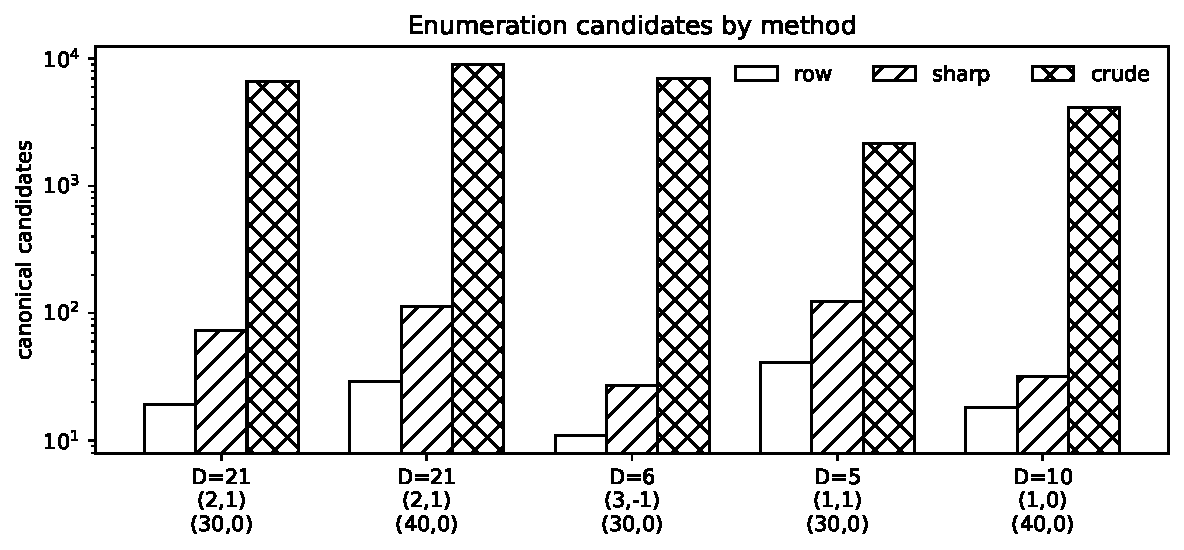
\includegraphics[width=0.82\textwidth]{enumeration_candidates.pdf}
\caption{Canonical candidate counts on a logarithmic scale for the weighted-search benchmarks of Table~\ref{tab:enum}. The exact row search consistently stays below the sharp-box baseline and far below the deliberately crude box.}
\Description{Bar chart on a logarithmic vertical axis comparing exact row enumeration, sharp box, and crude box candidate counts. The exact row bars are lowest in every displayed benchmark.}
\label{fig:enumplot}
\end{figure}

Figure~\ref{fig:enumplot} visualises the same structural separation on a logarithmic scale. This is the software-facing interpretation of the ellipse-sensitive enumeration theorem: the exact row method improves the right candidate count, not merely the wall-clock time.

\begin{table}[tbp]
\centering
\tiny
\setlength{\tabcolsep}{2.0pt}
\begin{tabularx}{\textwidth}{c l c c l l c c r r r r r}
\toprule
$D$ & coeffs & $\alpha$ & ord & $|\cS_{a_i}(\alpha)|$ & DP states & left & right & pre & DPc & DPt & MITMc & MITt \\
\midrule
10 & $[(1,0),(4,1)]$ & $(18,2)$ & $[1,0]$ & $[1,5]$ & $[2,11]$ & 2 & 6 & 0.023 & 0.007 & 0.030 & 0.006 & 0.029 \\
5 & \shortstack[l]{$[(1,0),(1,0),$\\$(1,0)]$} & $(15,1)$ & \shortstack[l]{$[0,1,$\\$2]$} & \shortstack[l]{$[13,13,$\\$13]$} & \shortstack[l]{$[14,61,$\\$108]$} & 14 & 61 & 0.030 & 0.421 & 0.451 & 0.109 & 0.140 \\
21 & \shortstack[l]{$[(2,1),(1,0),$\\$(1,0),(1,0)]$} & $(30,0)$ & \shortstack[l]{$[1,2,$\\$3,0]$} & \shortstack[l]{$[12,12,$\\$12,13]$} & \shortstack[l]{$[13,60,$\\$131,195]$} & 60 & 95 & 0.059 & 1.114 & 1.180 & 0.181 & 0.240 \\
13 & \shortstack[l]{$[(1,0),(2,1),$\\$(2,1),(1,0)]$} & $(18,0)$ & \shortstack[l]{$[1,2,$\\$0,3]$} & \shortstack[l]{$[5,5,$\\$9,9]$} & \shortstack[l]{$[6,15,$\\$49,84]$} & 15 & 35 & 0.044 & 0.289 & 0.328 & 0.077 & 0.117 \\
\bottomrule
\end{tabularx}
\caption{Representability benchmarks. The ``ord'' column records the internal coefficient order used
by the implementation; the timing columns are split into preprocessing, DP-combination, DP-total,
meet-in-the-middle-combination, and meet-in-the-middle-total measurements.}
\label{tab:repr}
\end{table}

Table~\ref{tab:repr} makes the timing scope explicit. The preprocessing time is shared weighted-set
construction. The ``DPc'' and ``MITMc'' entries measure only the combination layers, whereas ``DPt''
and ``MITt'' are the full end-to-end routines. This is why the meet-in-the-middle speedup in the last
three examples remains visible even after the shared preprocessing is included.

\begin{table}[tbp]
\centering
\scriptsize
\begin{tabular}{c c c c r r r r}
\toprule
$D$ & $\alpha$ & ord & $|\prod_i V_i(\alpha)|$ & pre & DPt & MITt & generic \\
\midrule
10 & $(18,2)$ & $[1,0]$ & 12 & 0.027 & 0.034 & 0.034 & 0.031 \\
5 & $(15,1)$ & $[0,1,2]$ & 2744 & 0.034 & 0.481 & 0.151 & 0.717 \\
21 & $(30,0)$ & $[1,2,3,0]$ & 30758 & 0.068 & 1.259 & 0.242 & 9.727 \\
13 & $(18,0)$ & $[1,2,0,3]$ & 3600 & 0.046 & 0.343 & 0.127 & 1.203 \\
\bottomrule
\end{tabular}
\caption{Surrogate general-purpose exact baseline for single-target representability. The ``generic'' column expands the full Cartesian product of the value lists after the same exact preprocessing used by DP and meet-in-the-middle.}
\label{tab:generic}
\end{table}

Table~\ref{tab:generic} is the TOMS-facing comparison point. The artefact does not depend on an
external CAS, so instead of timing SageMath or PARI/GP directly we bundle a reproducible generic
exact baseline that mirrors the post-enumeration task a general-purpose system would still have to
solve: given the exact weighted-value sets, search their full Cartesian product for a representation.
This keeps the comparison portable while still showing the algorithmic advantage of reusing partial
sums. The structural column $|\prod_i V_i(\alpha)|$ records the raw search size of that baseline.

\begin{figure}[tbp]
\centering
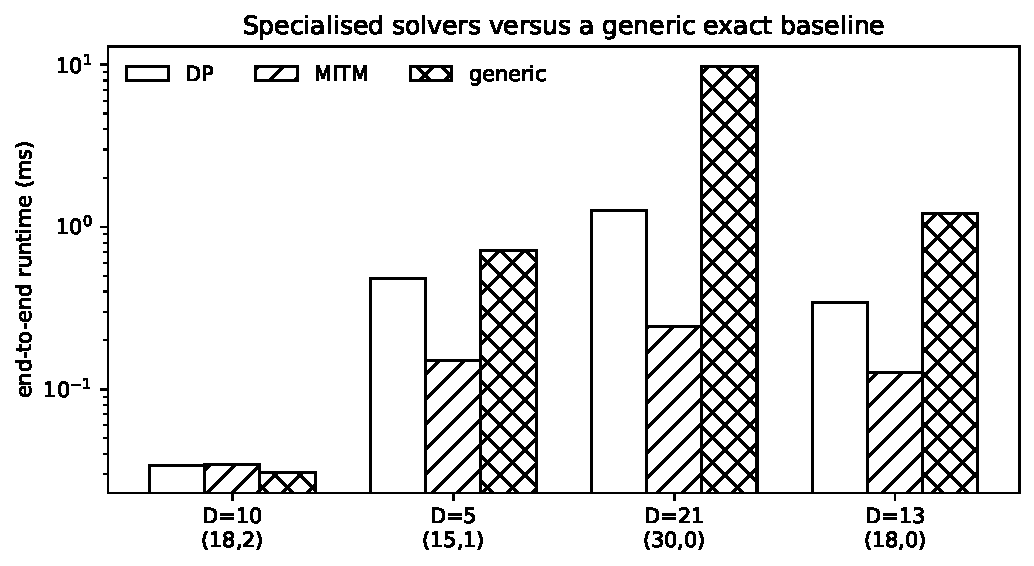
\includegraphics[width=0.74\textwidth]{generic_baseline_runtime.pdf}
\caption{End-to-end runtimes for constructive DP, meet-in-the-middle, and the bundled generic exact baseline of Table~\ref{tab:generic}. The specialised solvers exploit partial-sum reuse, whereas the generic baseline expands the full Cartesian product of the value lists.}
\Description{Log-scale bar chart comparing dynamic programming, meet-in-the-middle, and generic baseline runtimes. The generic baseline grows fastest on larger examples.}
\label{fig:generic}
\end{figure}

As a concrete constructive witness, for $D=5$, $L=\langle (1,0),(1,0),(1,0)\rangle$, and
$\alpha=(15,1)$, the dynamic program returns the root tuple
\[
\bigl((0,1),(-1,2),(3,0)\bigr),
\]
hence the explicit representation
\[
(15,1)
=
(1,0)(0,1)^2 + (1,0)(-1,2)^2 + (1,0)(3,0)^2
=
(1,1)+(5,0)+(9,0).
\]
This illustrates that the implementation is genuinely constructive: it returns actual roots, not
merely a yes/no answer.

\begin{table}[tbp]
\centering
\tiny
\setlength{\tabcolsep}{2.0pt}
\begin{tabularx}{\textwidth}{c l c c l l r r r r}
\toprule
$D$ & coefficients & $\alpha$ & ord & original states & optimised states & pre$_\mathrm{unc}$ & pre$_\mathrm{c}$ & DP$_\mathrm{orig}$ & DP$_\mathrm{opt}$ \\
\midrule
10 & $[(1,0),(4,1)]$ & $(18,2)$ & $[1,0]$ & $[6,11]$ & $[2,11]$ & 0.020 & 0.019 & 0.029 & 0.027 \\
13 & \shortstack[l]{$[(1,0),(2,1),$\\$(2,1),(1,0)]$} & $(18,0)$ & \shortstack[l]{$[1,2,$\\$0,3]$} & \shortstack[l]{$[10,31,$\\$49,84]$} & \shortstack[l]{$[6,15,$\\$49,84]$} & 0.083 & 0.033 & 0.365 & 0.313 \\
21 & \shortstack[l]{$[(2,1),(1,0),$\\$(1,0),(1,0)]$} & $(30,0)$ & \shortstack[l]{$[1,2,$\\$3,0]$} & \shortstack[l]{$[14,95,$\\$190,195]$} & \shortstack[l]{$[13,60,$\\$131,195]$} & 0.088 & 0.046 & 1.499 & 1.038 \\
\bottomrule
\end{tabularx}
\caption{Coefficient-order and repeated-coefficient optimisation. The timing columns record,
respectively, uncached preprocessing, cached preprocessing, original end-to-end DP runtime, and
optimised end-to-end DP runtime.}
\label{tab:opt}
\end{table}

Table~\ref{tab:opt} illustrates the practical value of
Proposition~\ref{prop:ordering-upper} and Proposition~\ref{prop:caching}. Sorting by
non-decreasing weighted-set size reduces the intermediate DP upper bound and, in practice, the DP
state counts as well, while repeated-coefficient caching reduces preprocessing when a coefficient
occurs more than once. The second row is typical: the two repeated coefficients $(2,1)$ are
preprocessed only once, and the internal ordering cuts the first two DP layers from $[10,31]$ to
$[6,15]$.

\begin{figure}[tbp]
\centering
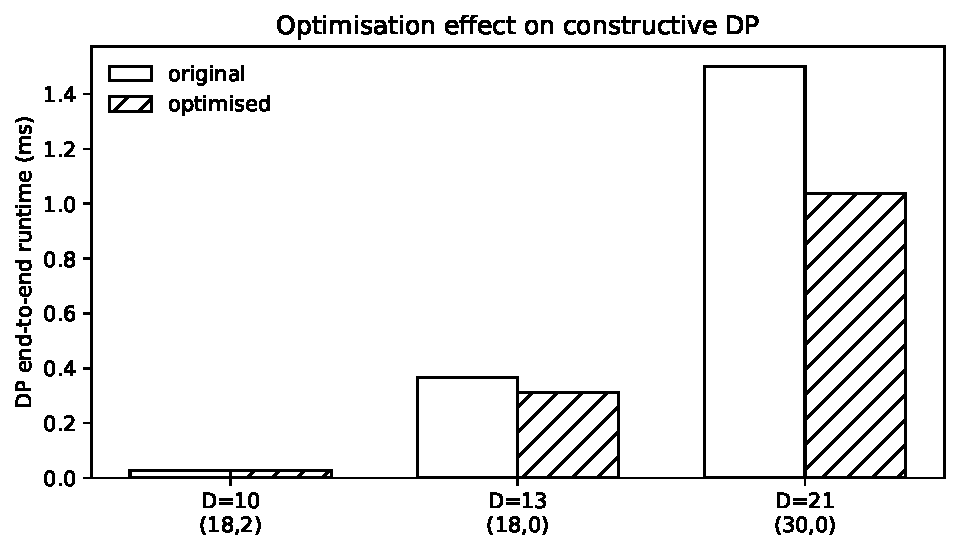
\includegraphics[width=0.72\textwidth]{optimisation_runtime.pdf}
\caption{End-to-end constructive DP runtimes before and after internal coefficient reordering and repeated-coefficient caching for the optimisation benchmarks of Table~\ref{tab:opt}.}
\Description{Bar chart comparing original and optimised constructive dynamic-programming runtimes. The optimised variant is lower in each benchmark.}
\label{fig:optplot}
\end{figure}

\begin{table}[tbp]
\centering
\tiny
\begin{tabular}{clrrrrcc}
\toprule
$D$ & coefficients & $B$ & represented & truants & $|\cW_i(B)|-1$ & batched states & times (ms) \\
\midrule
5 & $[(1,0),(1,0),(1,0)]$ & 10 & 25 & 0 & $[7,7,7]$ & $[8,20,26]$ & $0.010/0.065/0.112/0.685$ \\
10 & $[(1,0),(4,1)]$ & 18 & 6 & 21 & $[1,3]$ & $[2,7]$ & $0.011/0.004/0.043/0.604$ \\
21 & $[(2,1),(1,0),(1,0)]$ & 16 & 23 & 7 & $[4,6,6]$ & $[5,18,24]$ & $0.016/0.047/0.105/0.998$ \\
\bottomrule
\end{tabular}
\caption{Batched bounded search versus per-target recomputation. The timing column lists, in order,
batched preprocessing, batched dynamic-programming combination, full batched end-to-end runtime, and
full naive end-to-end runtime.}
\label{tab:bounded}
\end{table}

Table~\ref{tab:bounded} illustrates the algorithmic gain from
Theorem~\ref{thm:pseudopoly}. The structural columns show that the batched routine works with the
bounded value sets $\cW_i(B)$ and the intermediate bounded state sets $\cQ_j(B)$ exactly as the
proof predicts. The timing column shows the important comparison: the full batched end-to-end
routine is already substantially faster than solving each target separately, even at these modest
bounds.

\begin{figure}[tbp]
\centering
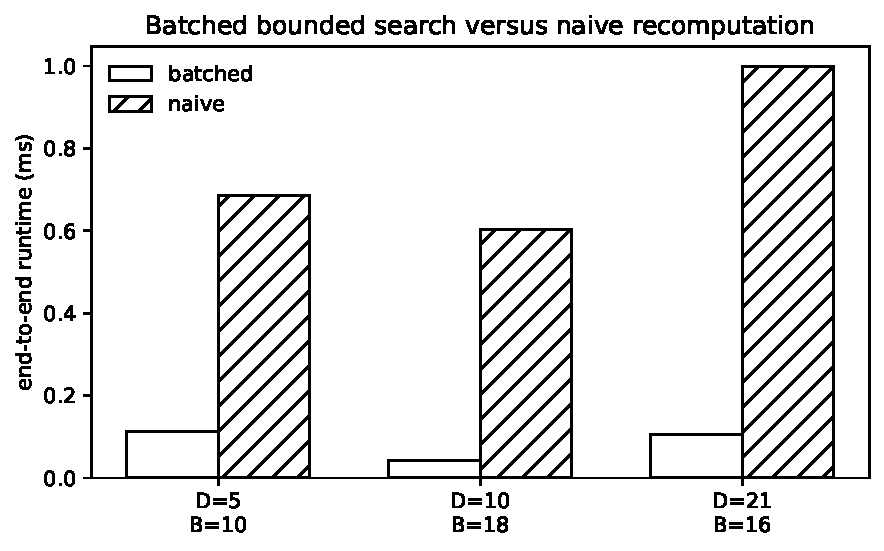
\includegraphics[width=0.74\textwidth]{bounded_runtime.pdf}
\caption{End-to-end runtimes for the batched bounded routine and naive per-target recomputation in Table~\ref{tab:bounded}. The important comparison is the full batched end-to-end runtime versus the full naive end-to-end runtime.}
\Description{Bar chart comparing batched bounded search with naive per-target recomputation. Batched search is lower for all displayed cases.}
\label{fig:boundedplot}
\end{figure}

\begin{table}[tbp]
\centering
\scriptsize
\begin{tabularx}{\textwidth}{c l c X}
\toprule
$D$ & coefficients & $B$ & bounded truant set \\
\midrule
5 & $[(1,0),(1,0),(1,0)]$ & 12 & none \\
5 & $[(1,0),(1,0),(2,1)]$ & 40 & none \\
13 & $[(1,0),(2,1),(2,1),(1,0)]$ & 18 & $[(3,-1),(3,0),(3,2),(6,-1),(6,3)]$ \\
21 & $[(2,1),(1,0),(1,0)]$ & 16 & $[(4,2),(6,-2),(5,2),(6,0),(7,-2),(6,2),(8,-2)]$ \\
\bottomrule
\end{tabularx}
\caption{Explicit bounded truant sets computed by the batched algorithm.}
\label{tab:arith}
\end{table}

Table~\ref{tab:arith} is the first genuine arithmetic output of the note: explicit bounded truant
profiles for several real-quadratic lattices. The second row corresponds to the classical ternary
lattice
\[
\langle 1,1,(5+\sqrt5)/2\rangle,
\]
written in the basis $\{1,\omega_5\}$ as coefficients $[(1,0),(1,0),(2,1)]$; the absence of bounded
truants up to trace bound $40$ is consistent with the known universality picture over $\Q(\sqrt5)$
\cite{KalaSurvey}. The \(D=13\) row is especially compact and illustrates the usefulness of the
batched method when the coefficient list contains repetitions. The bundled notebook reproduces this
table, the balancing example above, and the optimisation diagnostics from Table~\ref{tab:opt}.

For an explicit omission witness, take $D=21$, $L=\langle (2,1),(1,0),(1,0)\rangle$, and
$\alpha=(4,2)$, which is the first truant in the last row of Table~\ref{tab:arith}. Here
\[
\cS_{(1,0)}(\alpha)=\varnothing,
\qquad
\cS_{(2,1)}(\alpha)=\{(2,1)\}.
\]
In the internally reordered coefficient order $[1,2,0]$, the value lists are therefore
\[
V_1(\alpha)=V_2(\alpha)=\{0\},
\qquad
V_3(\alpha)=\{0,(2,1)\}.
\]
Hence the dynamic-programming state sets are
\[
P_1(\alpha)=\{0\},
\qquad
P_2(\alpha)=\{0\},
\qquad
P_3(\alpha)=\{0,(2,1)\},
\]
so $\alpha\notin P_3(\alpha)$ and therefore $\alpha\nrightarrow L$. This is a typical explicit
non-representability certificate produced by the same infrastructure.

\section{Concluding remarks}

The paper is deliberately positioned as a computational number-theory contribution rather than as a
classification paper. Its novelty lies in the exact real-quadratic specialisation and integration of
weighted lattice enumeration, constructive diagonal representability, coefficient-order optimisation,
and batched bounded search. The arithmetic examples above show that the infrastructure already yields
explicit bounded truant data.

Several natural extensions suggest themselves. First, one can replace the diagonal weighted-value
sets by bounded sections of more general positive definite lattices and ask for a batched bounded
search for non-diagonal forms. Second, extending the framework to non-maximal orders would require a
careful treatment of the conductor and modified coordinate models, but the present exact comparison
machinery should still be relevant there. Third, extending beyond real quadratic fields would force a
qualitative change in the geometry: in degree $d>2$ the weighted trace form becomes a positive-definite
lattice problem in rank $d$, so for cubic fields the search region is an ellipsoid in $\R^3$ and the
exact row-interval formulas and canonical half-ellipse scan used here no longer suffice. Fourth, the
current routines are designed to be used as a subroutine in diagonal escalator and criterion-set
computations of the type considered by Kala--Kr\'asensk\'y--Romeo \cite{KKR}. Finally, the present
DP and meet-in-the-middle state-count bounds are purely combinatorial; it would be interesting to
sharpen them by exploiting additional multiplicative structure inside $\OD^+$.


\bibliographystyle{ACM-Reference-Format}
\bibliography{references}

\end{document}
